\section{The sharp chain law}\label{sec:law}

Theorems~\ref{thm:xx-full-law} and~\ref{cor:ising-full-law} concern the exact finite spectra. Their common mechanism is a smooth limit of logarithmic Schmidt rank, with quantitative control of every spectral plateau. We first prove a criterion that isolates this mechanism.

\paragraph{Energy counts and logarithmic rank.}
Consider a family of spectra written as $p_\nu=e^{-L(1)-A_\nu}$,
where $A_\nu\ge0$ are energies listed with multiplicity and
$L(z)=\log\sum_\nu e^{-z A_\nu}$ is the logarithm of the partition
function. Under the tilted law $p_{\beta,\nu}=e^{-L(\beta)-\beta A_\nu}$,
the mean and variance of $A$ are $m_\beta=-L'(\beta)$ and
$v_\beta=L''(\beta)$. In particular $V=v_1$ is the information
variance of the original spectrum. Let $W\to\infty$ index the family.

\begin{proposition}[A counting criterion for the embezzlement law]
\label{prop:xx-count-to-error}
Suppose $L$ is analytic on a fixed complex neighborhood of a fixed
real interval $[1-\eta,1+\eta]\subset(0,\infty)$, with
$|L^{(k)}(z)|\le C_k W$ for each fixed $k\ge1$, and $v_\beta\ge cW$
on the real interval. Suppose the tilted characteristic functions
$\varphi_\beta(t)=\mathbb E_\beta e^{itA}$ obey, uniformly in that interval,
\begin{equation}\label{eq:chain-damping}
 |\varphi_\beta(t)|\le
 \begin{cases}
 e^{-cWt^2}, & |t|\le\delta,\\
 e^{-cW}, & \delta\le |t|\le\tau W,
 \end{cases}
\end{equation}
for positive constants $c,\delta,\tau$ independent of $W$. Then, for all
integers $d\ge2$, with $h=\log d$,
\begin{equation}\label{eq:xx-error-capacity}
 \left|\mathcal E_d-\frac{h^2}{4V}\right|
 \le\frac{C(1+h^2+h^4)}{W^2}.
\end{equation}
Here $C$ and the large-$W$ threshold are independent of $d$.
\end{proposition}

\begin{proof}
Write $R(E)=\#\{\nu:A_\nu\le E\}$ and
$R(E^-)=\#\{\nu:A_\nu<E\}$. Set $\mu=m_1$ and $B=\sqrt W\log W$.
For $|E-\mu|\le2B$, let $\beta(E)$ solve $m_\beta=E$. Since
$m_\beta'=-v_\beta$ has magnitude of order $W$, this solution is unique
and lies in the given interval for large $W$. Define
\begin{equation}\label{eq:xx-saddle-F}
 F(E)=L(\beta(E))+\beta(E)E-\log\beta(E)
      -\tfrac12\log(2\pi v_{\beta(E)}).
\end{equation}
Lemma~\ref{lem:xx-microscopic-counting} in Appendix~\ref{app:xx-full}
gives the uniform estimate for $|E-\mu|\le2B$,
\begin{equation}\label{eq:xx-microscopic-counting}
 \log R(E)=F(E)+O(W^{-1}),\qquad
 \log R(E^-)=F(E)+O(W^{-1}).
\end{equation}
Indeed, with $\beta=\beta(E)$ the exact tilted count is
\[
 e^{-L(\beta)-\beta E} R(E)=\mathbb E_\beta
      \bigl[e^{-\beta(E-A)}\mathbf1_{\{A\le E\}}\bigr].
\]
The lemma uses both frequency bounds in~\eqref{eq:chain-damping} and
an even smoothing kernel with Fourier support in $[-\tau W,\tau W]$.
The tilted interval-probability estimate~\eqref{eq:xx-concentration}
bounds the change under smoothing and the mass of any atom at $E$
by $O(W^{-3/2})$. The analytic derivative bounds and $v_\beta\asymp W$
give the saddle-point value $(\beta\sqrt{2\pi v_\beta})^{-1}$ with
relative error $O(W^{-1})$ in the Fourier integral
\eqref{eq:xx-smoothed-fourier}.

Put $p(x)=p_{\lceil x\rceil}$ for the decreasing list of probabilities,
with zero padding for a finite list, and $g(y)=e^{y/2}\sqrt{p(e^y)}$.
If $E_x=-\log p(x)-L(1)$ is finite, then
$R(E_x^-)<x\le R(E_x)$. The two counts in
\eqref{eq:xx-microscopic-counting} give $\log x=F(E_x)+O(W^{-1})$
throughout each degenerate plateau in the counting window.
Since $F'(E)=\beta(E)+O(W^{-1})$ is bounded away from zero there,
its inverse $E_*(y)=F^{-1}(y)$ satisfies the energy
comparison~\eqref{eq:xx-inverse-rank} on
$F([\mu-3B/2,\mu+3B/2])$. Let $\chi$ be a smooth function equal to one
on $[-1,1]$ and supported inside $(-3/2,3/2)$, and define
\[
 G(y)=\chi\bigl((E_*(y)-\mu)/B\bigr)
        \exp\bigl((y-L(1)-E_*(y))/2\bigr)
\]
on the range of $F$, extended by zero. Lemma~\ref{lem:chain-rank-profile}
proves
\begin{equation}\label{eq:chain-profile-estimates}
 \norm{g-G}_2=O(W^{-1}),\qquad \norm{G''}_2=O(W^{-1}),\qquad
 \norm{G'}_2^2=\frac{1}{4V}+O(W^{-2}).
\end{equation}
The first estimate uses concentration under the original law to control
the full tail. The derivative estimates follow from the logarithmic
derivative $a(E)=1-1/F'(E)$ of the squared uncut profile. Its Taylor
coefficients about $\mu$ through degree two have orders
$O(W^{-1})$, $-1/V+O(W^{-2})$, and $O(W^{-2})$, respectively.
The first and third centered moments of the exact energy are $0$ and
$O(W)$, which controls the cross terms in the integral of $a^2$.

For $T_h g(y)=g(y-h)$ set $D_h=I-T_h$. The continuous rank coordinate
preserves the exact error $\mathcal E_d=\norm{D_hg}_2^2$ because
$p(x/d)=p_{\lceil j/d\rceil}$ almost everywhere on $(j-1,j]$.
Writing $r=g-G$, we have
\[
 \norm{D_hg}_2^2-\norm{D_hG}_2^2
   =2\operatorname{Re}\langle D_h^*D_hG,r\rangle+\norm{D_hr}_2^2.
\]
The multiplier of $D_h^*D_h=2I-T_h-T_{-h}$ is $2-2\cos(ht)$, bounded
by $h^2t^2$. Thus the last display is $O((1+h^2)W^{-2})$ by
\eqref{eq:chain-profile-estimates}. The same multiplier differs from
$h^2t^2$ by $O(h^4t^4)$, so
$\norm{D_hG}_2^2=h^2\norm{G'}_2^2+O(h^4\norm{G''}_2^2)$.
This proves~\eqref{eq:xx-error-capacity}.
\end{proof}

\paragraph{The exact covariance supplies the counting estimates.}
For the open XX chain let $C_N$ be the occupied one-particle projector
and write $C_N$ in blocks for the two halves. If $s_j$ are the singular
values of its cross block, then $s_j^2=\lambda_j(1-\lambda_j)$ as a
multiset, where $\lambda_j$ are the restricted covariance eigenvalues.
The Schmidt probabilities form a product of two-outcome distributions
with one-mode energies $e_j=2\operatorname{arcosh}(1/(2s_j))$.
With zero padding, Corollary~\ref{cor:xx-mesh} compares the ordered
$(s_j)$ in $\ell^1$ with error $O(1)$ to the mesh
\begin{equation}\label{eq:chain-main-mesh}
 \left\{\tfrac12\operatorname{sech}(2\pi^2 k/L_i)
                    :k\in\mathbb Z,\ i=1,2\right\},
 \qquad L_i=\log N+O(1).
\end{equation}
The two branches come from the two parity blocks of the exact sine
covariance. Each is compared with a finite Hilbert matrix, then with a
periodized Carleman kernel diagonal in Fourier modes.

This mesh gives $\sum_j s_j=O(\log N)$, which bounds the fixed-order
derivatives of $L(z)=\sum_j\log(1+e^{-ze_j})$ by $O(\log N)$ near
$\beta=1$. In any fixed positive energy band $[a,b]$, a mesh branch
has spacing $4\pi^2/L_i$. All but $O(1)$ entries in the band match
true energies in $[a/2,2b]$, with total absolute discrepancy $O(1)$.
These modes give $v_\beta\ge c\log N$. The Bernoulli characteristic
factor has squared modulus $1-4q(1-q)\sin^2(te_j/2)$, where
$q=(1+e^{\beta e_j})^{-1}$. For small $t$ the retained modes give a
sine-square sum of order $Wt^2$ with $W=\log N$. For $|t|\ge\delta$
the mesh sum is bounded below by $cW-O(1+|t|)$ by integral comparison.
Replacing the mesh energies by the matched true energies costs another
$O(1+|t|)$. Choosing $\tau$ sufficiently small yields
\eqref{eq:chain-damping} through $|t|\le\tau W$.

The entropy and information variance are sums over modes of
\[
 f_S(e)=\log(1+e^{-e})+\frac{e}{1+e^e},\qquad
 f_V(e)=\frac{e^2 e^e}{(1+e^e)^2}.
\]
As functions of $s=(2\cosh(e/2))^{-1}$ both are Lipschitz. The mesh
comparison therefore changes their sums by $O(1)$. The two mesh
branches give density $(L_1+L_2)/(2\pi^2)$ in positive energy and
$\int_0^\infty f_S(e)\,de=\int_0^\infty f_V(e)\,de=\pi^2/6$.
This gives~\eqref{eq:xx-three-limits} and recovers the open-boundary
entropy coefficient of Calabrese and Cardy and of Fagotti and
Calabrese for XX~\cite{CalabreseCardy04,FagottiCalabrese11}.
The matching leading term for $V$, the capacity of entanglement,
agrees with the conformal R\'enyi calculation~\cite{deBoer19,Arias23}.
Proposition~\ref{prop:xx-count-to-error} now gives
\eqref{eq:xx-full-rate} and~\eqref{eq:xx-full-limit}.

For Ising, the exact Majorana decomposition identifies the mode list of
the XX chain on $2L$ sites with two copies of the Ising list on $L$
sites (Corollary~\ref{cor:ising-fourier}). The Ising logarithmic partition
function is therefore half that of XX, and its tilted characteristic
function has modulus equal to the square root of the XX modulus. This
proves Corollary~\ref{cor:ising-full-law} with $W=\log L$.

\begin{corollary}[Loss of the explicit strategy]\label{cor:xx-strategy}
For the finite open XX and critical Ising states, the explicit
measurements of Theorem~\ref{thm:operational-upper} achieve
$\mathcal B(p)=(2/243)\mathcal E_2(1+o(1))$. The leading losses are
$(\log2)^2/(81\log N)$ for XX and $2(\log2)^2/(81\log L)$ for Ising.
\end{corollary}

\begin{proof}
The same mesh gives $b_N=-\log p_1\sim(\log N)/12$ for XX and
$b_L\sim(\log L)/24$ for Ising (Appendix~\ref{app:xx-full}). Thus
$p_1=o(\mathcal E_2)$, and the achieved loss follows from the
state-dependent estimate in Theorem~\ref{thm:operational-upper}.
\end{proof}

Corollary~\ref{cor:chain-arbitrary-cuts} extends the chain law uniformly
to cuts between any two adjacent sites in either open chain as the
shorter side grows. The logarithm of the shorter side sets the scale.
The corollary also covers Ising chains of odd length.

\begin{corollary}[Targets of growing dimension]\label{cor:chain-growing-target}
Under the assumptions of Proposition~\ref{prop:xx-count-to-error},
uniformly over integers $d\ge2$ as $W\to\infty$,
\begin{equation}\label{eq:chain-gaussian-crossover}
 \mathcal E_d=2\left(1-\exp\left[-\frac{(\log d)^2}{8V}\right]\right)+o(1).
\end{equation}
In particular the error tends to zero precisely when $\log d=o(\sqrt V)$.
In this regime the error is asymptotic to $(\log d)^2/(4V)$ by
\eqref{eq:xx-error-capacity}.
\end{corollary}

The optimal local-unitary root fidelity $1-\mathcal E_d/2$ has the
limiting Gaussian form proved for LOCC by Zhang, Liu and
Chen~\cite[Supplement, Theorem~1]{ZhangLiuChen26}. The counting criterion
establishes this form for the exact finite XX and Ising spectra.

\begin{proof}
Set $y_0=F(\mu)=L(1)+\mu-\tfrac12\log(2\pi V)$ and define the
probability density $\rho_W(z)=\sqrt V\,g(y_0+\sqrt V\,z)^2$.
For $y=y_0+\sqrt V\,z$ at fixed $z$, let $u=F^{-1}(y)-\mu$.
Since $F'$ is bounded away from zero, $u=O_z(\sqrt W)$.
The derivative bounds from Appendix~\ref{app:xx-full} give
\[
 F(\mu+u)-F(\mu)=u-\frac{u^2}{2V}
              +O\left(\frac{|u|}{W}+\frac{|u|^3}{W^2}\right).
\]
It follows that $u=\sqrt V\,z+O_z(1)$. By the inverse count estimate
\eqref{eq:xx-inverse-rank}, the exact energy at rank $e^y$ is
$\mu+u+O(W^{-1})$. Consequently
\[
 \log\rho_W(z)=-\tfrac12\log(2\pi)+y-y_0-u+O(W^{-1})
              \longrightarrow-\tfrac12\log(2\pi)-z^2/2.
\]
Both $\rho_W$ and the standard normal density $\phi$ integrate to one.
Dominated convergence applied to $\min(\rho_W,\phi)$ gives
$\norm{\rho_W-\phi}_1\to0$ and hence
$\norm{\sqrt{\rho_W}-\sqrt\phi}_2\to0$. Translation by $h$ in $y$
becomes translation by $h/\sqrt V$ in $z$. Since $\norm{I-T_a}\le2$
uniformly in real $a$, the squared translation errors of the two
square-root densities differ by $o(1)$ uniformly in the shift.
The Gaussian overlap is
$\langle\sqrt\phi,T_a\sqrt\phi\rangle=e^{-a^2/8}$, which gives
\eqref{eq:chain-gaussian-crossover}.
\end{proof}

\subsection{Exact discrete towers}

For an end block of a critical chain, conformal field theory describes the
reduced state through an annulus Hamiltonian. Its width grows as
$W=\ln(\kappa N)$ and its level degeneracies depend on the boundary
operator content~\cite{PeschelEisler09,Lauchli13,CardyTonni16,ACT18}.
For the corresponding open-boundary conformal comparison, the free-fermion
towers have odd one-body levels
\begin{equation}\label{eq:levels}
\varepsilon_\ell=(2\ell+1)\varepsilon,\qquad
\varepsilon=\pi^2/W,
\end{equation}
once for Ising and twice for XX~\cite{IgloiJuhasz08}. The double odd tower
is the comparison for the XX sizes divisible by four used in the numerical
study. When $N/2$ is odd, the finite XX covariance has an exact $1/2$ mode,
which contributes a flat Schmidt factor. The finite-chain theorem
covers both parity sectors. Such towers also occur
as exact half-chain spectra in integrable gapped models~\cite{PKL99}.
For the towers themselves, the leading embezzlement law can be proved
without replacing the discrete levels by a smooth density.
For a fixed integer $r\geq1$ and $\varepsilon>0$, consider the normalized
countable spectrum
\begin{equation}\label{eq:tower-spectrum-rigorous}
 p_{\boldsymbol\nu}=Z_r(\varepsilon)^{-1}
 \exp\!\left[-\varepsilon
   \sum_{a=1}^{r}\sum_{\ell\geq0}(2\ell+1)\nu_{a,\ell}\right],
 \qquad
 Z_r(\varepsilon)=\prod_{\ell\geq0}
       (1+e^{-(2\ell+1)\varepsilon})^r .
\end{equation}
Here every $\nu_{a,\ell}$ is $0$ or $1$ and only finitely many occupations
are nonzero.  Order the probabilities decreasingly as $(p_j)_{j\geq1}$,
put $\lambda_j=\sqrt{p_j}$, and define
\[
 (D_d\lambda)_j=d^{-1/2}\lambda_{\lceil j/d\rceil},
 \qquad
 \mathcal E_d=\norm{\lambda-D_d\lambda}_2^2,
 \qquad S=-\sum_j p_j\log p_j .
\]
The cases $r=1,2$ are the single and double odd-level towers used for
the Ising and XX conformal spectra, respectively.

\begin{theorem}[Exact discrete tower law]\label{thm:exact-tower-law}
Fix integers $r\geq1$ and $d\geq2$, and set
$c_r=r\pi^2/24$.  For the exact spectrum
\eqref{eq:tower-spectrum-rigorous}, as $\varepsilon\downarrow0$,
\begin{align}
 S&=\frac{2c_r}{\varepsilon}+O_r(\varepsilon),
 \label{eq:tower-entropy-rigorous}\\
 \mathcal E_d
 &=\frac{(\log d)^2\varepsilon}{8c_r}
       +O_{r,d}(\varepsilon^2),
 \label{eq:tower-error-rigorous}\\
 \mathcal E_d S&=\frac{(\log d)^2}{4}
       +O_{r,d}(\varepsilon).
 \label{eq:tower-product-rigorous}
\end{align}
All constants are independent of $\varepsilon$. The left-hand sides use
the exact discrete spectrum with its full level multiplicities.
\end{theorem}


Appendix~\ref{app:tower} proves the tower law by applying
Proposition~\ref{prop:xx-count-to-error} to the exact spectrum with
$W=\varepsilon^{-1}$. The tilted characteristic-function
bound~\eqref{eq:characteristic-tail} for the integer tower levels
gives~\eqref{eq:chain-damping} after rescaling to the physical energy
spacing. This yields the $O_{r,d}(\varepsilon^2)$ remainder.
Lemma~\ref{lem:tower-uniform-comparison} also compares the exact tower
with the smooth Calabrese--Lefevre distribution in Hellinger distance.


\subsection{Numerical comparison}
For target dimension two, write $\cE_{\mathrm{tower}}^{(r)}(b)$ for the
$r$-copy tower curve at $b=-\ln p_1$, and $\cE_{\mathrm{s}}(b)$ for
the smooth Calabrese--Lefevre curve. The tower superscript labels level
multiplicity; the subscript $d$ in $\cE_d$ always labels the target dimension.

\begin{figure}[t]
\centering
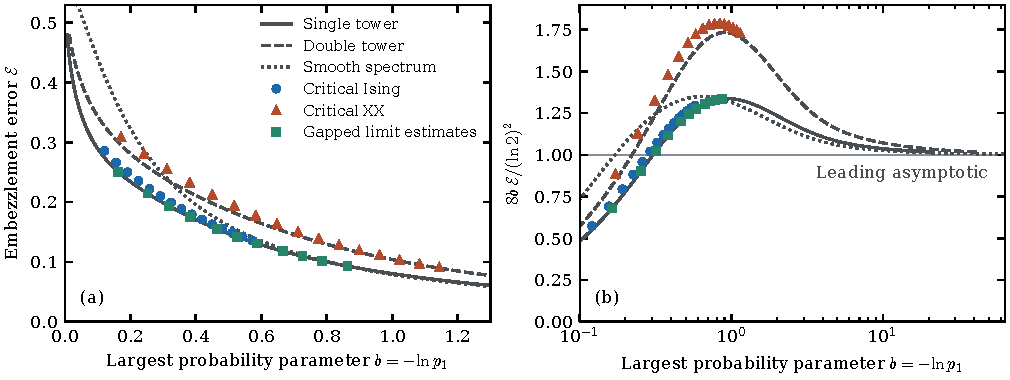
\includegraphics[width=\textwidth]{fig_law.pdf}
\caption{The finite-size law. (a) Embezzlement error against $b=-\ln p_1$ for the critical Ising
chain ($8$ to $131{,}072$ spins), the critical XX chain ($8$ to $262{,}144$ sites) and gapped
chains in the limit of long chains. Curves: prediction from equally spaced entanglement
levels~\eqref{eq:levels}, each level occurring once or twice, and from the smooth conformal
spectrum of Ref.~\cite{CalabreseLefevre08}. (b) The same data and curves multiplied by
$8b/(\ln2)^2$. The proved XX, Ising and tower asymptotics correspond to the value one; it is approached
slowly.}
\label{fig:law}
\end{figure}

\paragraph{Test.} We computed the entanglement spectra of the ground states of three chains by
the correlation-matrix method~\cite{Peschel03,VLRK03}: the critical XX chain with open ends, the
critical transverse-field Ising chain with open ends, and the XX chain with a staggered
potential, which is gapped with correlation length $\xi$. All chains are cut in the middle.
Appendix~\ref{app:numerics} gives the methods and checks. Figures~\ref{fig:main}(b)
and~\ref{fig:law} and Table~\ref{tab:chains} show the results.

\begin{table}[t]
\centering\small
\begin{tabular}{@{}llccccc@{}}
\toprule
 & & $S$ & $b$ & $\cE$ & $\cE/\cE_{\mathrm{tower}}^{(r)}(b)$ & $\cE/\cE_{\mathrm{s}}(b)$\\
\midrule
Critical Ising & $N=16$ & 0.423 & 0.156 & 0.2663 & 1.049 & 0.72 \\
 & $N=256$ & 0.663 & 0.292 & 0.2100 & 1.043 & 0.84 \\
 & $N=4{,}096$ & 0.895 & 0.419 & 0.1708 & 1.030 & 0.91 \\
 & $N=65{,}536$ & 1.126 & 0.542 & 0.1420 & 1.022 & 0.95 \\
 & $N=131{,}072$ & 1.184 & 0.572 & 0.1361 & 1.021 & 0.96 \\
\addlinespace
Critical XX & $N=16$ & 0.714 & 0.241 & 0.2799 & 1.065 & 0.97 \\
 & $N=256$ & 1.210 & 0.518 & 0.1935 & 1.065 & 1.24 \\
 & $N=4{,}096$ & 1.674 & 0.775 & 0.1382 & 1.038 & 1.33 \\
 & $N=65{,}536$ & 2.136 & 1.022 & 0.1034 & 1.020 & 1.34 \\
 & $N=262{,}144$ & 2.367 & 1.144 & 0.0908 & 1.015 & 1.34 \\
\addlinespace
Staggered XX & $\xi=20$ & 0.729 & 0.318 & 0.1932 & 1.000 & 0.82 \\
 & $\xi=200$ & 1.114 & 0.526 & 0.1420 & 1.000 & 0.93 \\
 & $\xi=2{,}000$ & 1.498 & 0.726 & 0.1092 & 1.000 & 0.98 \\
 & $\xi=10{,}000$ & 1.766 & 0.864 & 0.0929 & 1.000 & 1.00 \\
\bottomrule
\end{tabular}
\caption{Entanglement entropy $S$, $b=-\ln p_1$ and embezzlement error $\cE$ of half-chain
ground states. $\cE_{\mathrm{tower}}^{(1)}$ (Ising and gapped chains) and $\cE_{\mathrm{tower}}^{(2)}$ (XX chain) are the predictions from
equally spaced levels at the same $b$; $\cE_{\mathrm{s}}$ is the prediction of the smooth
conformal spectrum. For gapped chains the values estimate the long-chain limits.}\label{tab:chains}
\end{table}

In both critical chains $\cE$ decreases monotonically over the sampled
powers of two, spanning more than four decades in size. At the larger
sizes, the increments in $1/\cE$ grow with successive doublings.
The slope of $S$ with respect to $\ln N$ at the largest sampled
doubling is $0.083335$ for Ising and $0.166670$ for XX, close to $c/6$
for $c=1/2$ and $c=1$, respectively.

The spectra have the predicted form. For the gapped chain the one-body entanglement energies
satisfy $\varepsilon_\ell/\varepsilon_0=2\ell+1$ to five digits, and $\cE$ agrees with $\cE_{\mathrm{tower}}^{(1)}(b)$
within $2\times10^{-4}$ for all $\xi$ from $4$ to $10^4$. At criticality the levels are equally
spaced only approximately. For the Ising chain, expressing $\varepsilon_0$
as $\pi^2/\ln(\kappa N)$ gives $\kappa=16.9$ at $1{,}024$ spins and
$17.6$ at $131{,}072$ spins. The ratios
$\varepsilon_\ell/\varepsilon_0$ for $\ell=1,2,3$ are $3.13$, $5.46$ and $7.95$
at $1{,}024$ spins and $3.04$, $5.18$ and $7.39$ at $131{,}072$ spins.
Accordingly $\cE/\cE_{\mathrm{tower}}^{(1)}(b)$ falls from $1.05$ to $1.021$ for the Ising chain, and
$\cE/\cE_{\mathrm{tower}}^{(2)}(b)$ falls from $1.07$ to $1.015$ for the XX chain.

The comparison with the smooth spectrum shows which conformal data matter. At fixed $b$ the smooth spectrum is a one-parameter approximation that suppresses tower degeneracies, and at the largest sizes the XX chain lies $34\%$ above it
while the Ising chain lies $4\%$ below. What distinguishes $\cE_{\mathrm{tower}}^{(1)}$, $\cE_{\mathrm{tower}}^{(2)}$ and
$\cE_{\mathrm{s}}$ is the operator content, that is, the degeneracies of the levels of $L_0$.

The sampled chains remain pre-asymptotic for $\cE$. At $N=4{,}096$,
the XX chain gives $\cE\simeq0.13824$ and $V\simeq1.58147$.
The error is about $82\%$ above the capacity expression
$(\ln2)^2/(4V)\simeq0.07595$ and about $60\%$ above the leading
logarithmic expression $3(\ln2)^2/(2\ln N)\simeq0.08664$ in
\eqref{eq:xx-full-rate}.
The combination $8b\,\cE/(\ln2)^2$, which tends to one under
Theorem~\ref{thm:xx-full-law}, still equals $1.19$, $1.08$ and
$1.016$ at $b=2$, $4$ and $16$ for the smooth spectrum, and $1.14$ and $1.27$ at $b=3.2$ on the
curves $\cE_{\mathrm{tower}}^{(1)}$ and $\cE_{\mathrm{tower}}^{(2)}$.
The Ising and XX samples reach $b=0.57$ and $b=1.14$, respectively.
On the large-$S$ side of Figure~\ref{fig:diagnostics}(a), the
entropy-normalized error comes within ten per cent of one near
$S\simeq7$ for the smooth curve and near $S\simeq9$ and $S\simeq15$
for the single and double towers.

Gapped chains behave like critical chains of finite length. Their $\cE$ stops decreasing once
$N$ exceeds a few correlation lengths (Figure~\ref{fig:main}(b)). The estimated limiting value lies close to
the curve $\cE_{\mathrm{tower}}^{(1)}(b)$ and falls slowly with $\xi$, from $0.193$ at $\xi=20$ to $0.142$, $0.109$
and $0.093$ at $\xi=200$, $2{,}000$ and $10{,}000$.


\begin{figure}[t]
\centering
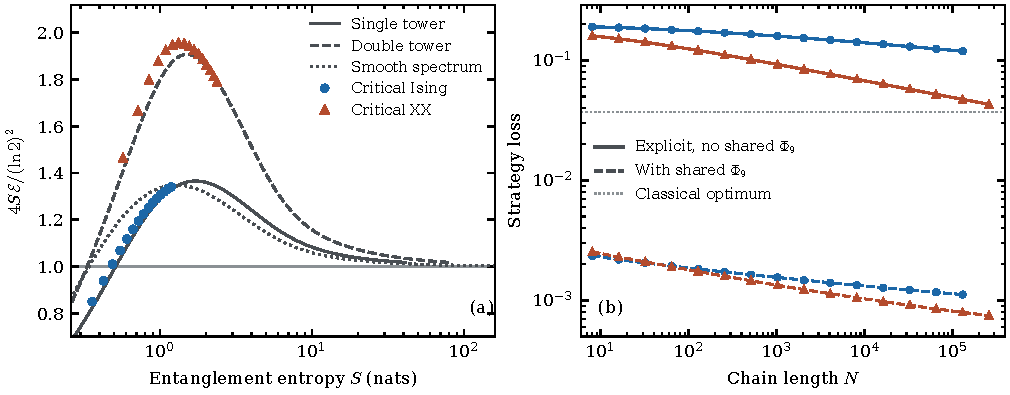
\includegraphics[width=\textwidth]{fig_diagnostics.pdf}
\caption{(a) The entropy-normalized error for the physical chains, exact
towers and smooth spectrum. The exact tower and finite-chain theorems give limit one.
(b) The exact loss of the explicit unassisted strategy (solid) and the
loss after adding $\Phi_9$ (dashed). The horizontal line is the classical
optimum $1/27$. These are achieved strategy losses, not values of the
optimization over all measurements.}\label{fig:diagnostics}
\end{figure}

At the largest sizes the explicit unassisted losses are $0.11895$ for Ising
and $0.04295$ for XX, both above the classical loss $1/27$.
With the additional $\Phi_9$, the losses are $1.120\times10^{-3}$ and
$7.472\times10^{-4}$. These achieved losses lie below the classical bound and above the flat-spectrum
floor $\gamma$. The compressed certificate of
Section~\ref{sec:xx84-separation} establishes separation in the original
game at the explicit larger length $N=2^{84}$.
Section~\ref{sec:finite-chain-hybrid} gives an exact four-spin separation
using a tagged extension, and Section~\ref{sec:operational-lower} gives
a nine-qubit resource separated by the original game.
